\begin{frame}{Dateiformat}
	\begin{block}{Warum überhaupt ein Dateiformat?}
		\begin{itemize}
			\pause
			\item unabhängige Komponenten
			\item klar definierte Schnittstelle
		\end{itemize}
	\end{block}
	\pause
	\begin{block}{Vorteile}
		\begin{itemize}
			\pause
			\item unabhängiges Arbeiten
			\item Teamaufteilung
			\pause
			\item Darstellung austauschbar
			\item einmaliges Datensammeln
			\pause
			\item GUI-Entwicklung in Java
		\end{itemize}
	\end{block}
\end{frame}

\begin{frame}<1-2>[label=overview]{Überblick}
	\begin{block}{Elemente}
		\begin{itemize}
			\pause
			\item Datei-Header
			\pause
			\item Matrizen-Header
			\pause
			\item Matrizen-Informations-Block
			\pause
			\begin{itemize}
				\item Bytearrays
				\pause
				\item Zugriffsarten
				\pause
				\item Zugriffspattern
				\pause
				\item Zugriffssequenz
				\pause
				\item Name
			\end{itemize}
		\end{itemize}
	\end{block}
\end{frame}

\begin{frame}[fragile,squeeze]{Details}
	\begin{block}{Matrizen-Header}
		{\fontsize{6}{6}\selectfont
		\begin{verbatim}
			+---+---+---+---+---+---+---+---+---+---+---+---+---+---+---+---+---+---+---+---+
			|  SX   |  SY   |NLA|NSA|NAP|NSQ|              ADR              |     MIBADR    |
			+---+---+---+---+---+---+---+---+---+---+---+---+---+---+---+---+---+---+---+---+
			|     SLH       |      SLM      |      SSH      |      SSM      |
			+---+---+---+---+---+---+---+---+---+---+---+---+---+---+---+---+
		\end{verbatim}
		}
	\end{block}
	\begin{block}{Elemente}
		\begin{itemize}[<+->]
			\pause
			\item Größe der Matrix: SX (Size X), SY (Size Y)
			\item Anzahl zugehöriger Elemente: NLA (Number of Loading Accesses), NSA (Number of Storing Accesses), NAP (Number of Accesss Patterns), NSQ (Number of access SeQuences)
			\item Kosmetisches: ADR (ADRess), MDBADR (MDB ADRess)
			\item statistische Daten zur Matrix: SLH (Sum Load Hits), SLM (Sum Load Misses), SSH (Sum Store Hits), SSM (Sum Store Misses)
		\end{itemize}
	\end{block}
\end{frame}

\againframe<2-8>{overview}

\newcommand{\puta}[3]{\begin{picture}(0,0)(0,0)\put(#1,#2){#3}\end{picture}}
\begin{frame}{Graphischer Überblick}
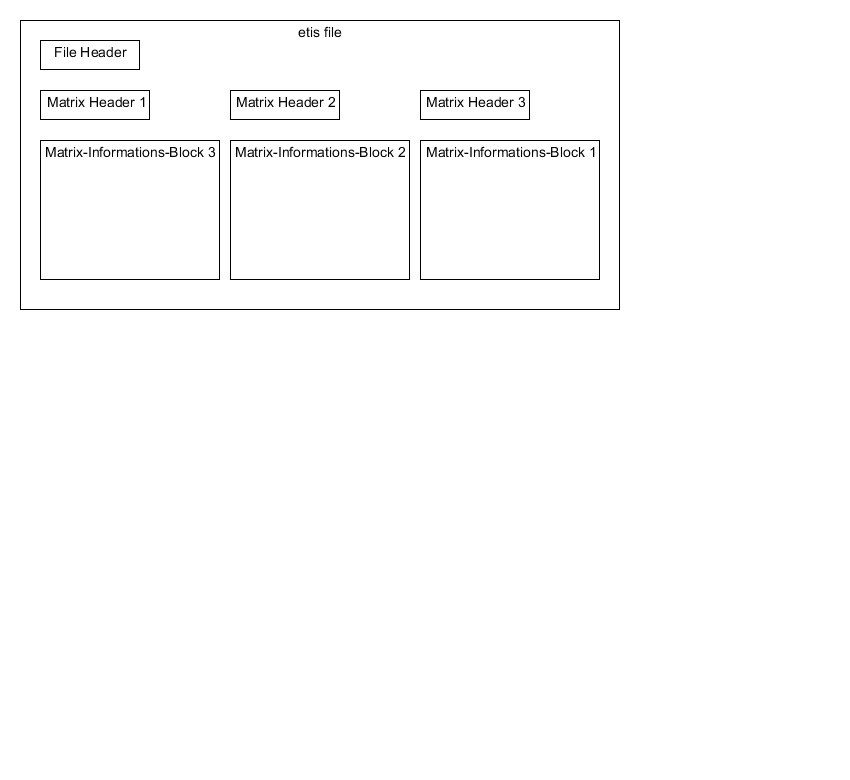
\includegraphics[height=0.95\textheight]{mctracer/dateiaufbau1}
\end{frame}

\begin{frame}{Graphischer Überblick}
 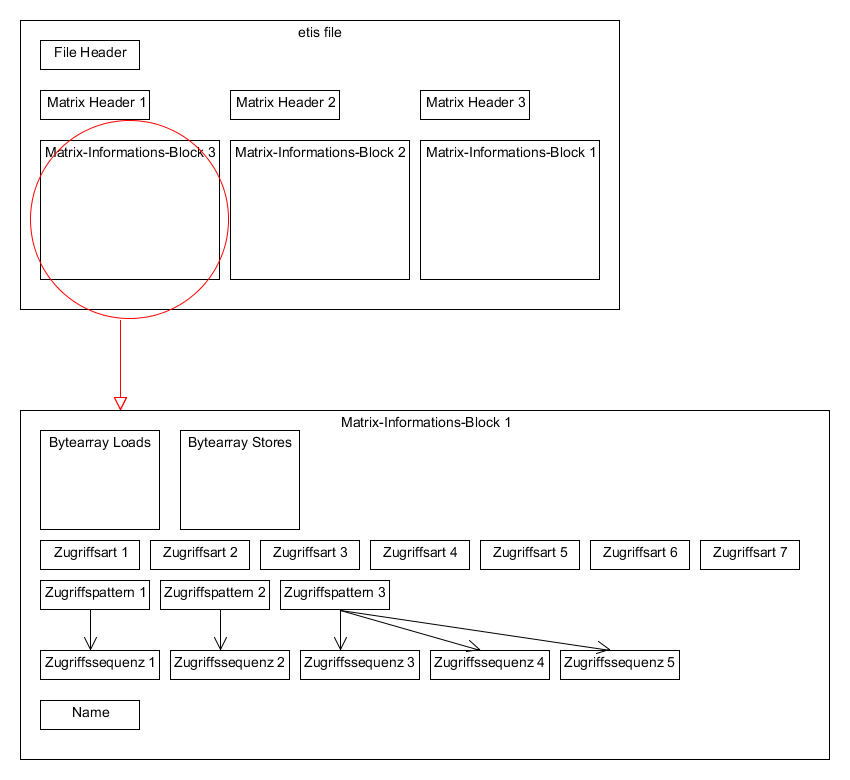
\includegraphics[height=0.95\textheight]{mctracer/dateiaufbau2}
\end{frame}

\begin{frame}{Graphischer Überblick}
 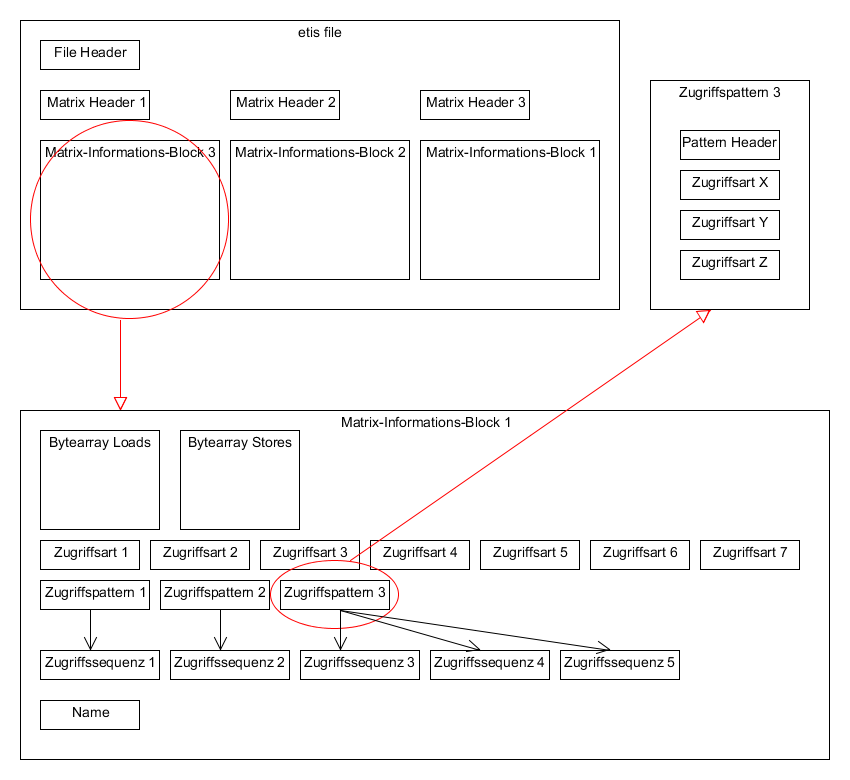
\includegraphics[height=0.95\textheight]{mctracer/dateiaufbau3}
\end{frame}